\chapter{Evaluation}
\label{chap:evaluation}
In this chapter, we aim to evaluate different aspects of the developed system. This includes a cost analysis, a performance analysis, and finally a field test of a simplified artwork tracking scenario.

\section{Cost and Performance Analysis}
The primary cost factor of the artis-system is the \gls{sc}. Each execution of a function that mutates the state of the \gls{sc} costs a certain amount of gas which in turn has a price in Ether. The cost for a transaction thus is calculated as follows:
$$
transaction\ fee = gas \times gas\ price
$$
To analyze the execution costs of the \textit{safeMint} and \textit{updateArtworkData} contract functions, we executed the corresponding requests of the developed \gls{api} multiple times $(n = 10)$ and recorded transaction fees as well as the request time in seconds. This analysis was conducted on the sepolia testnet and the resulting transactions were inspected on the Etherscan block explorer. The transactions were submitted with a relatively high gas price (30 Gwei) to make the transactions attractive for validators \cite{ethergas}.

\begin{figure}[ht]
    \begin{subfigure}{0.49\textwidth}
        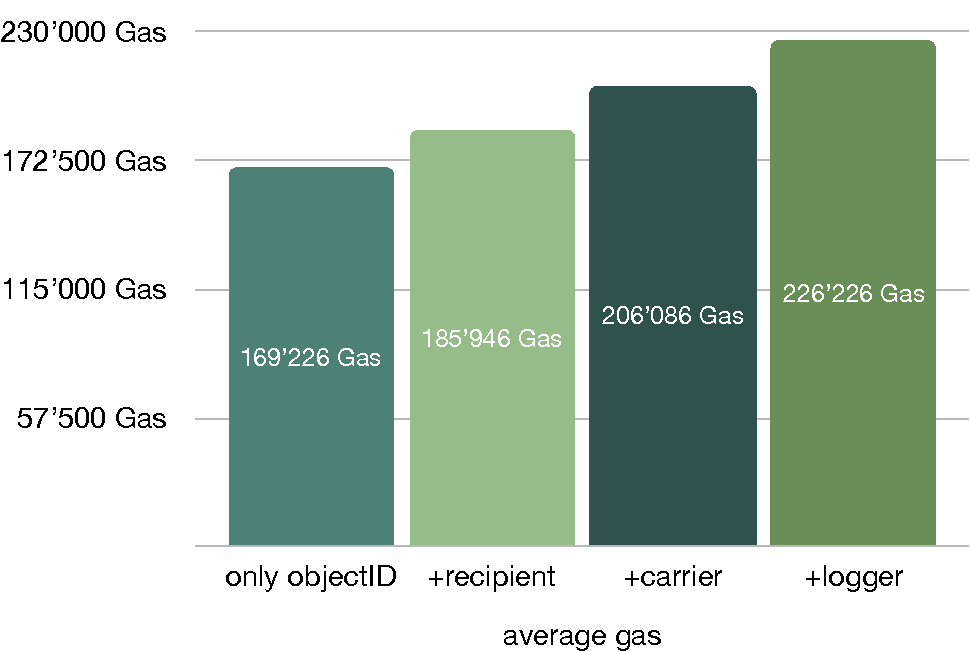
\includegraphics[width=\textwidth]{diagrams/safeMint_gas_eval.pdf}
        \caption{Transaction gas usage}
        \label{fig:safemint_tx_cost}
    \end{subfigure}
    \hfill
    \begin{subfigure}{0.49\textwidth}
        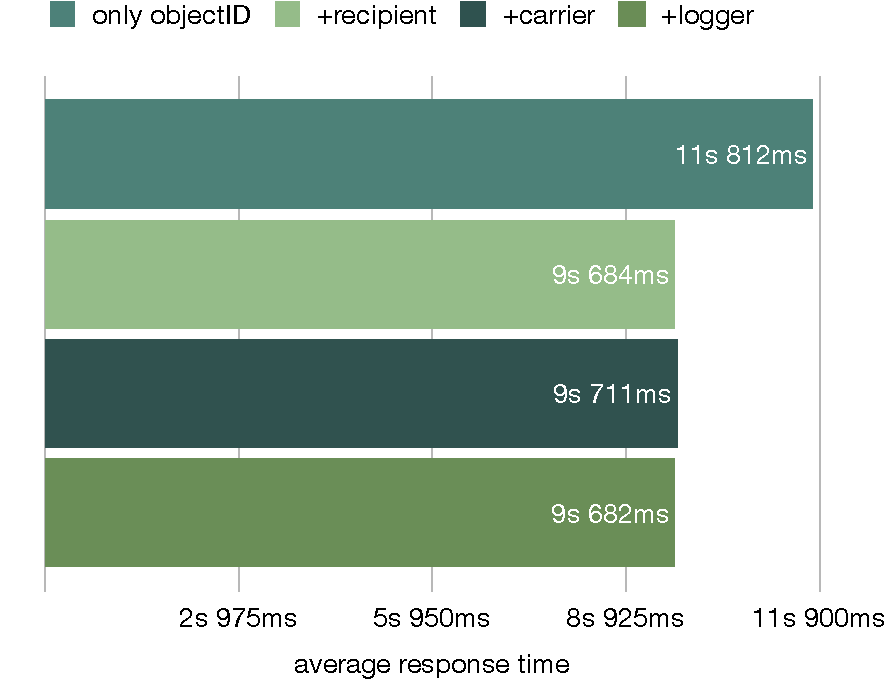
\includegraphics[width=\textwidth]{diagrams/safeMint_request_time_eval.pdf}
        \caption{Request speed in seconds}
        \label{fig:safemint_tx_speed}
    \end{subfigure}
    \caption{safeMint analysis}
    \label{fig:safemint_analysis}
\end{figure}

\subsection*{safeMint}
Figure \ref{fig:safemint_analysis} shows the average gas consumed by the safeMint function. Each bar shows the average of 10 function executions with varying parameters. On the very left is the average gas used if only the objectID of the artwork is added during minting. The second bar shows the gas consumed if the objectID and the recipient address are provided during minting. The analysis shows that the more parameters are provided the more gas it consumes.

\begin{table}[]
\begin{tabular}{cllll}
                                          & \textbf{only objectID} & \textbf{+recipient} & \textbf{+carrier} & \textbf{+logger} \\ \cline{2-5} 
\multirow{2}{*}{\textbf{Transaction fee}} & 0.0048 ETH             & 0.0053 ETH          & 0.0059 ETH        & 0.0064 ETH       \\
                                          & 7.71 CHF               & 8.47 CHF            & 9.39 CHF          & 10.31 CHF       
\end{tabular}
\caption{Transaction fees for safeMint}
\label{tab:safemint_tx_fees}
\end{table}

To get a sense of how gas translates into fees we used the average gas price for the Ethereum mainnet (28 Gwei) \cite{gaspriceaverage} and the current value of Ether in \gls{chf} (1599.32 CHF = 1 ETH) \cite{coinmarketcap}. The results are listed in Table \ref{tab:safemint_tx_fees}.


\subsection*{updateArtworkData}
Similarly, we also conducted an analysis of the updateArtworkData function. The bar on the very left of Figure \ref{fig:updateArtworkData_tx_cost} shows the average gas consumed by the function when updating the requested status on 10 \glspl{nft}. Approving the status as a different actor then shows an average gas consumption of 82'662. The last two bars show the gas amount for reporting a violation from the logger and registering a carrier. 


\begin{figure}[h]
    \begin{subfigure}{0.49\textwidth}
        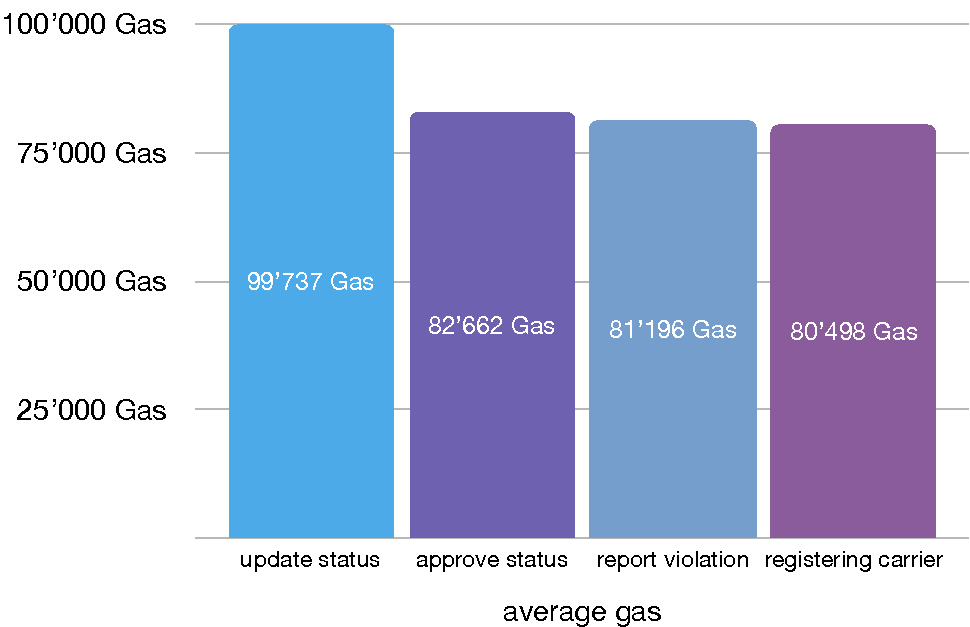
\includegraphics[width=\textwidth]{diagrams/updateArtworkData_gas_eval.pdf}
        \caption{Transaction gas usage}
        \label{fig:updateArtworkData_tx_cost}
    \end{subfigure}
    \hfill
    \begin{subfigure}{0.49\textwidth}
        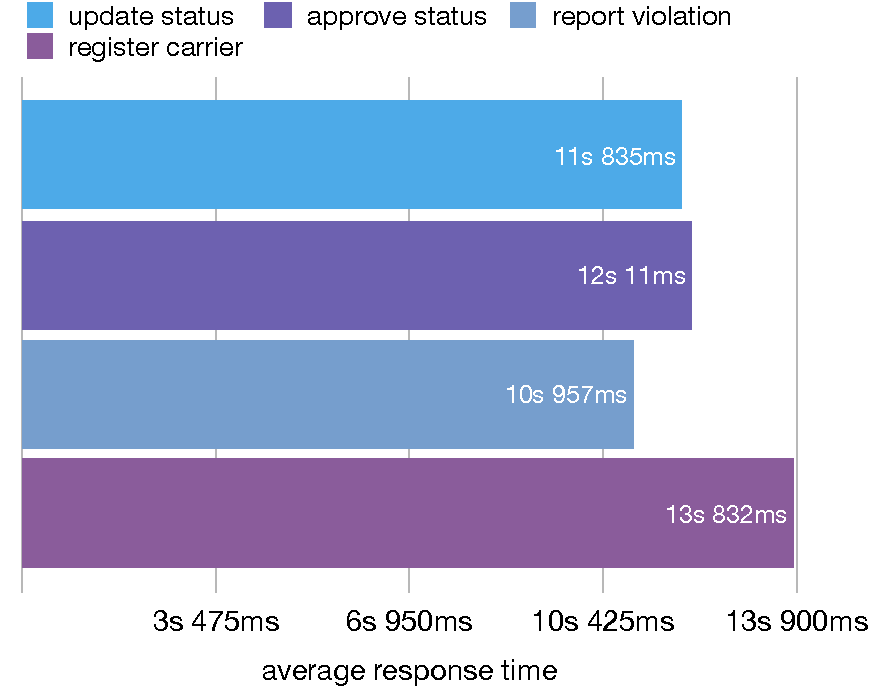
\includegraphics[width=\textwidth]{diagrams/updateArtworkData_request_time_eval.pdf}
        \caption{Request speed in seconds}
        \label{fig:updateArtworkData_tx_speed}
    \end{subfigure}
    \caption{updateArtworkData analysis}
    \label{fig:updateArtworkData_analysis}
\end{figure}

\begin{table}[ht]
\begin{tabular}{cllll}
                                          & \textbf{update status} & \textbf{approve status} & \textbf{report violation} & \textbf{register carrier} \\ \cline{2-5} 
\multirow{2}{*}{\textbf{Transaction fee}} & 0.0028 ETH             & 0.0024 ETH          & 0.0023 ETH        & 0.0023 ETH       \\
                                          & 4.54 CHF               & 3.77 CHF            & 3.70 CHF          & 3.67 CHF       
\end{tabular}
\caption{Transaction fees for updateArtworkData}
\label{tab:updateArtworkData_tx_fees}
\end{table}


\subsection*{Non-Mutating Functions}
The GET endpoints exposed by the \gls{api} target several functions that do not mutate the state of the \gls{sc}. These functions do not cost any gas and their execution time is much less (usually < 1 Second). Additionally, the artis-server adds a caching layer to these function calls which generally reduce the response time of repeated calls to a few milliseconds. 

\section{Field Test}
In addition to the above analyses, we also performed a simulated scenario of transporting an artwork. This test is composed of several steps:

\begin{enumerate}
    \item create a new artwork \gls{nft} and register the corresponding roles using the artis-frontend.
    \item request the status of the artwork to be changed to \textit{IN\_TRANSIT} from the sender account
    \item approve this request from the carrier account
    \item enable the logger by starting the \textit{logging\_script} and the \textit{violation\_script} with the thresholds of 27 degrees Celcius and 70\% humidity.
    \item take the logging device and transport it from point of departure to destination
    \item during the transportation simulate a violation by wrapping a hand around the sensor to increase the temperature.
    \item upon arrival request the status of the artwork to be changed to \textit{DELIVERED} from the carrier account
    \item approve this request from the recipient account
\end{enumerate}

%section discussion